\chapter{Using Kepler’s Laws to find the density of Jupiter}

%todo include caution about rotation of image compared to website
%todo give the density of water, to aid analysis of planet as rocky or gaseous

\section{Introduction}

So far, you have been using several techniques to learn about the properties of planets orbiting other stars based one what we can observe from Earth, including using orbital properties to discover the mass of planets. The same physical laws can be used to study planets and their moons.

To study the composition of a planet, it is useful to know its density --- then one can learn more about whether it is rocky or gaseous. In this lab, you will use Kepler's Laws to find the density of Jupiter, given orbital properties of its moons. In this case, we can use actual images of the these using Stone Edge Observatory, a remotely operated telescope in California.

Under nominal circumstances, we would have you schedule the observations yourself, so you could analyze the data that you, yourself, took. However, the observatory is not operating well enough right now to let that happen. Fortunately, we have archival images that were taken in 2017 by this observatory that you can analyze.

\section{Using Kepler's laws}

Keplers third law relates the orbital period to the systems semi-major axis. In the case where the planets mass is much smaller than the stars mass, Kepler's third law is:
\begin{equation}
P^2 = \frac{4\pi^2}{G M}a^2 \,,
\end{equation}
where $P$ is the orbital period, $G$ is Newton's constant ($6.674 \times 10^{11}\:\textrm{N}\:\textrm{m}^2/\textrm{kg}^2$), $M$ is the mass of Jupiter, and $a$ is the semi-major axis.

We can rewrite the third law as:

\begin{equation}
\frac{a^3}{P^2} = \frac{G}{4\pi^2}\left(\frac{4}{3}\pi R^3\rho \right) = \rho\frac{G R^3}{3\pi}
\end{equation}

where $R$ is the radius of Jupiter and $\rho$ (the Greek letter pronounced ``row'') is the density of Jupiter. Solving for $\rho$ gives:

\begin{equation}
\rho = \left(\frac{a}{R}\right)^3\frac{3\pi}{G P^2}
\end{equation}

The goal for this lab is to use our data to determine the ratio $(a/R)$ for each moon. We can then combine that with the moons period to estimate the density of Jupiter.

To determine the semi-major axis, $a$, for a moon's orbit, we can assume that the orbit is actually a circular orbit, and we know that we are viewing the orbits edge-on. So what we are seeing is a projection of a circular motion onto one dimension, which results in a sinusoidal motion, with the amplitude of that motion being the radius of the orbit (and thus the semi-major axis). So here we will analyze images taken at different times, plot the angular position of the moon over time, and fit those data points to a sine (or, equivalently, a cosine) function, and the amplitude will be the semi-major axis, $a$.

\section{The set of observations}

The images can be found on Canvas, in the Files section, in the compressed file ``jupiter\_data.zip''.

Observations were taken on four separate dates between April 14 and 23, 2017, as stated in the names of the files. Images were taken in each of the \textit{g}, \textit{r}, \textit{i}, and \textit{clear} bands. These refer approximately to the color filters used in each case: green, red, infrared, and  clear (no filter). See Figure~\ref{jd:fig:filters} for the frequency response of such a filter set. All images were taken with a $0.05\:$second exposure time.

\begin{figure}
	\centering
	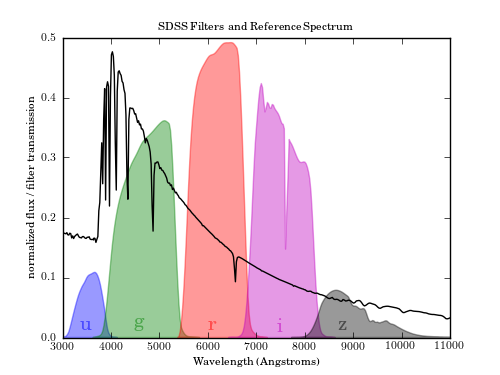
\includegraphics[width=0.8\textwidth]{jupiter-density/fig_sdss_filters_1}
	\caption{Typical transmission rates of various filters used in astronomy. This is from the Sloan Digital Sky Survey.}\label{jd:fig:filters}
\end{figure}

%\section{Make color images}
%
%All CCDs which are used in astronomical images are monochrome --- they do not have different pixels for different wavelengths of light, which allows them to achieve higher resolution. To create a color image, we must combine the images taken with different color filters and add color ourselves.
%
%One can easily make RGB images in DS9 by selecting \textit{Frame} $>$ \textit{New Frame RGB}, which allows one to upload different .fits files for each color with \textit{File} $>$ \textit{Open} depending on the color selected in the pop-up window. You can then scale each image as needed to make 3-color images. \textbf{Make an RGB image for Jupiter.}
%
\section{Analysis}

You will use the \textit{clear} images to measure the position of the moons relative to Jupiter and
\textit{gri} images to measure the radius of Jupiter. Since we will be using the ratio of moon position to Jupiter radius, we can use whatever units are convenient to measure the distance, as long as we are consistent, as the unit divides by itself in the calculation.

\begin{steps}
	\item \textbf{Use} DS9 to load and analyze each of the FITS files. To get a better view, select ``Scale >> Log'' from the drop-down menus. Using the Ruler function (described in the following paragraph), \textbf{for each timestamp, estimate the radius} of Jupiter from the \textit{i}-filter file (where available) \textbf{and the position} of each moon relative to Jupiter from the \textit{clear}-filter file. Keep track of whether the moon is on the East or West side of Jupiter by making all locations on the East side positive and locations on the West side negative.
\end{steps}

You can use the DS9 \textit{Ruler} function to measure the distance (in pixels) between two points in the image. To use the \textit{Ruler}, first go to the Region menu from the toolbar at the top. Select the \textit{Shape} sub-menu and click \textit{Ruler}. Then, click the \textit{Edit} menu button and select \textit{Region}. You can then use the mouse to draw a line between two points and DS9 will calculate the distance for you. If you have trouble using the \textit{Ruler} feature, you can also read off the $(x,y)$ coordinates for each point and calculate the distance yourself. \textbf{Record your values} in a data table in a spreadsheet.

\begin{steps}
	\item \textbf{Record the time} the image was taken by going to the \textit{File} menu and then \textit{Display Fits Header}. Towards the bottom of the header will be listed the \textit{DATE-OBS} which will be in UTC time. To identify each moon at the time of the picture, use the following site: \url{http://www.shallowsky.com/jupiter/}, be sure to enter the correct date into the site. 

	\item For each moon, find the semi-major axis of its orbit by fitting a sine curve to the data, using the following procedure:

	\begin{enumerate}
		\item Copy your data into a new table in SciDAVis. It should have the time in days (include fraction of days) in the $x$ column and the $x/R$ ratio in the $y$ column. For your report, format the table and graph according to Appendix~\ref{cha:lab-report-format}.
		
		\item Use SciDAVis to fit the following function to the data:
		\begin{equation}
		 X_i = A \cos \left( \frac{2\pi T_i}{P} + \phi \right)\,.
		\end{equation}
		Here, $X_i$ is the position of the moon scaled to the radius of Jupiter, $A$ the amplitude of the sinusoid, which corresponds to the corresponds to the orbit semi-major axis divided by $R_\textrm{Jupiter}$, $T_i$ the time of the observation, $P$ the period of the moon's orbit, and $\phi$ the phase of the orbit. $X_i$ and $T_i$ are the data you obtain with your observations, and $A$ and $\phi$ are the parameters you will fit. Enter the period for the relevant moon from Table~\ref{jd:tab:periods}.
	\end{enumerate}
\end{steps}

\begin{table}
	\centering
	\begin{tabular}{ l c r }
		\hline
		Moon & Period (days) & $\rho_\textrm{Jupiter}$ $(\textrm{kg/m}^3)$\\
		\hline
		Ganymede & 7.1546 & \\
		Io & 1.7691 & \\
		Europa & 3.5512 & \\
		Calisto & 16.689 & \\
		\hline  
	\end{tabular}
	\caption{Four moons of Jupiter and their periods.}\label{jd:tab:periods}
\end{table}

The amplitude from your fit corresponds to the ratio, $(a/R)$ which we will use in Kepler’s Third law.

\begin{steps}
	\item For each moon, use the amplitude of the curve together with Keplers Third law
	to estimate the density of Jupiter. Make sure you use the right units for your values. \textit{Hint:
	look at the units for the Gravitational constant. What units do you need for the moons
	orbital period?}

	\item\label{jd:step:density} Take the average of the densities, and use the standard deviation of them for the uncertainty. Report this value, with uncertainty, in your report.
	
	\item Compare your result to a value of the density you find online, using the uncertainties and the procedure in Appendix~\ref{unc:sec:comparing}. How close are they? What are possible sources of uncertainty of your measurement?
	
	\item\label{jd:step:composition} Rocky planets in our solar system have densities ranging from 3000--5000$\:$kg/m$^3$. Given this and your result, would you conclude that Jupiter is rocky or gaseous, and why?
\end{steps}

\section{Report checklist and grading}

Each item below is worth 10 points, and there is an additional 10 points for attendance and participation.

\begin{enumerate}
	\item Data table including times and positions for each moon, as well as the radius of Jupiter.
	
	\item Graphs of position ($x/R$) vs. time for each moon, with the fitted curve plotted as well.
	
	\item Answers or evidence of completion for Steps~\ref{jd:step:density}--\ref{jd:step:composition}.
	
	\item A 100--200 word reflection on group dynamics and feedback on the lab manual. Address the following topics: who did what in the lab, how did you work together, what successes and challenges in group functioning did you have, and what would you keep and change about the lab write-up?
	
\end{enumerate}